\documentclass{standalone}
\usepackage{tikz}
\usepackage{ctex,siunitx}
\usepackage{tkz-euclide}
\usepackage{amsmath}
\usetikzlibrary{patterns, calc}
\usetikzlibrary {decorations.pathmorphing, decorations.pathreplacing, decorations.shapes,}
\begin{document}
\small
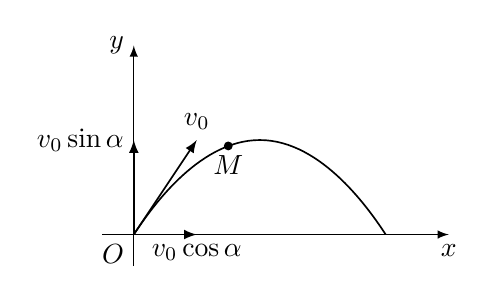
\begin{tikzpicture}[>=latex,scale=0.8]
  \tkzDefPoints{0/0/O,4/0/A,2/1.5/B,1/1.5/C}
  \draw[thin,->](-0.5,0)--(5,0)node[below]{$x$};
  \draw[thin,->](0,-0.5)--(0,3)node[left]{$y$};
  \draw [semithick](O) parabola bend (B)(A);
  \draw [semithick,->](O)--(C)node[above]{$v_0$};
  \draw [semithick,->](O)--(1,0)node[below]{$v_0\cos\alpha$};
  \draw [semithick,->](O)--(0,1.5)node[left]{$v_0\sin\alpha$};
  \fill (1.5,1.40625) circle(2pt)node[below]{$M$};
  \tkzLabelPoints[below left](O)
\end{tikzpicture}
\end{document}